%! Author = mariuszindel
%! Date = 02.11.20

\section{Klassen \& Structs}

\subsection{Klassen}
\begin{itemize}
    \item Reference Type $\rightarrow$ Auf dem Heap angelegt
    \item Vererbung
    \begin{itemize}
        \item Ableitung von Basisklasse möglich
        \item Implementation von Interfaces möglich
    \end{itemize}
    \item wird mit new instanziiert
    \item Deklaration
    \begin{itemize}
        \item Konstruktoren: Parameter optional
        \item Felder: Initialisierung erlaubt
    \end{itemize}
\end{itemize}

\begin{lstlisting}
class Stack {
    int[] values;
    int top = 0;

    public Stack(int size) { /* ... */ }

    public void Push(int x) { /* ... */ }
    public int Pop() { /* ... */ }
}
\end{lstlisting}

\subsection{Structs}
\begin{itemize}
    \item Value Type $\rightarrow$ Auf dem Stack angelegt oder «in-line» in einem Objekt auf dem Heap
    \item Vererbung
    \begin{itemize}
        \item Ableiten von Basisklasse nicht möglich
        \item Implementation von Interfaces möglich
    \end{itemize}
    \item wird mit new instanziiert
    \item Deklaration
    \begin{itemize}
        \item Konstruktoren: mind. 1 Parameter
        \item Felder: Initialisierung nicht erlaubt!
    \end{itemize}
\end{itemize}

\begin{lstlisting}
struct Point {
    int x;
    int y;

    public Point(int x, int y) {
        this.x = x; this.y = y;
    }
    public void MoveX(int x) { /* ... */ }
    public void MoveY(int y) { /* ... */ }
}
\end{lstlisting}

Ein Struct sollte nur unter folgenden Umständen verwendet werden:
\begin{itemize}
    \item Repräsentiert einen einzelnen Wert
    \item Instanzgrösse ist kleiner als 16 Byte (128 Bit)
    \item Ist “immutable”
    \item Wird nicht häufig geboxt
    \item Kurzlebig oder in andere Objekte eingebettet
\end{itemize}

In allen anderen Fällen sollte eine Klasse verwendet werden!

\subsubsection{Felder}
\begin{itemize}
    \item Initialisierung in Deklaration optional (ausser Struct)
    \item In Deklarationsreihenfolge initialisiert
    \item Initialisierung darf nicht auf Felder und Methoden zugreifen
    \item Struct-Felder dürfen nicht initialisiert werden
    \item Konstante muss Initialisierungswert haben und zur Compilezeit berechenbar sein
\end{itemize}

\begin{lstlisting}
class MyClass {
    int value = 0;
    const long size = int.MaxValue / 3 + 1234;
    readonly DateTime date1 = DateTime.Now;
    readonly DateTime date2;

    public MyClass() {
        date2 = DateTime.Now;
    }

    public void DoSomething() {
        value = 10;
        date2 = DateTime.Now; // Compilerfehler
    }
}
\end{lstlisting}


\subsubsection{Nested Types}
Für spezifische Hilfsklassen gedacht. Regeln:
\begin{itemize}
    \item Äussere Klasse hat Zugriff auf innere Klasse $\rightarrow$ Nur auf «Public Members»
    \item Innere Klasse hat Zugriff auf äussere Klasse $\rightarrow$ Auch auf «Private Members»
    \item Fremde Klassen erhalten Zugriff auf innere Klasse, wenn diese «public» ist
    \item Erlaubte Nested Types sind: Klassen, Interfaces, Structs, Enums, Delegates
\end{itemize}
\begin{lstlisting}
class OuterClass {
    private int outerValue;
    InnerClass innerInstance = new InnerClass();

    public void OuterMethod()
    { innerInstance.InnerMethod(this); }

    public class InnerClass {
        public void InnerMethod(OuterClass outerClass)
        { outerClass.outerValue = 123; } }
    }

// Anwendung
OuterClass outer = new OuterClass();
outer.OuterMethod();

OuterClass.InnerClass inner = new OuterClass.InnerClass();
inner.InnerMethod(outer);
\end{lstlisting}


\subsection{Methoden}
\subsubsection{Parameter Arten}
\paragraph{call by value}
\begin{itemize}
    \item Value-Parameter (call by value)
    \item Kopie des Stack-Inhaltes wird übergeben (Wert oder Heap-Referenz)
\end{itemize}
\begin{lstlisting}
void IncVal(int x) { x = x + 1; } void TestIncVal()
{
int value = 3;
IncVal(value); // value == 3 }
\end{lstlisting}

\paragraph{ref (call by reference)}
\begin{itemize}
    \item ref-Parameter (call by reference)
    \item Adresse der Variable «value» wird übergeben
    \item Variable «value» muss initialisiert sein
    \item Es muss eine Variable übergeben werden
\end{itemize}
\begin{lstlisting}
void IncRef(ref int x) { x = x + 1; } void TestIncRef()
{
int value = 3;
IncRef(ref value); // value == 4
    // Praxisbeispiel (Initialisierungen)
VectorStruct v = new VectorStruct();
    SetToZero(ref v);
}
\end{lstlisting}


\paragraph{out}
\begin{itemize}
    \item Wie ref-Parameter, aber zur Initialisierung von Werten gedacht
    \item Müssen initialisiert werden
    \item Darf in «Init» erst nach Wertzuweisung verwendet werden
    \item Variablen «a» / «b» dürfen initialisiert sein
    \item Nicht benötigte out-Parameter können mit Underscore «out \_» ignoriert werden
\end{itemize}


\begin{lstlisting}
void Init(out int a, out int b) { a = 1; b = 2; }

void TestInit() {

    // C# 7.0 regulaer
    Init(out int a1, out int b1); Console.WriteLine($"{a1} / {b1}");

    // C# 7.0 Parameter ignoriert
    Init(out int a2, out _); Console.WriteLine($"{a1}");
}
\end{lstlisting}

\paragraph{params}
Params-Array:
\begin{itemize}
    \item Erlaubt beliebig viele Parameter (0 – n)
    \item Muss am Schluss der Deklaration stehen
    \item Nur ein params-Array erlaubt
    \item Wird in «Sum» wie ein Array verwendet
    \item params darf nicht mit ref / out kombiniert werden
\end{itemize}
\begin{lstlisting}
void Sum(out int sum, params int[] values) {
    sum = 0;
    foreach (int i in values) sum += i;
}
\end{lstlisting}

\paragraph{OptionaleParameter}
\begin{itemize}
    \item Ermöglicht Zuweisung eines Default-Values
    \item Deklaration muss hinter erforderlichen Parametern erfolgen
    \item Muss zur Kompilierzeit berechenbar sein
    \item Weglassen nur am Ende erlaubt!
\end{itemize}
\begin{lstlisting}
private void Sort( int[] array, // Erforderlich
int from = 0,                   // Optional
int to = -1,                    // Optional
bool ascending = true,          // Optional
bool ignoreCase = false         // Optional
) { ... }
\end{lstlisting}


\subsection{Properties}
\begin{itemize}
    \item Kurzform für Get- / Set- Methoden
    \item Reines Compiler-Konstrukt
    \item Verhält sich wie «Public Field»
\end{itemize}

\begin{lstlisting}
class MyClass {
// Backing-Field
    private int length;
// Property
    public int Length
    {
        get { return length; }
        set { length = value; }
}
\end{lstlisting}
\subsection{Indexer}

Klasse verhält sich wie ein Array

\begin{lstlisting}
class MyClass {
    private string[] arr = new string[10];
    public string this[int index] {
        get { return arr[index]; }
        set { arr[index] = value; }
}

// Verwendung:
MyClass mc = new MyClass();
mc[0] = "Hello";
string value1 = mc[0]; // Hello
\end{lstlisting}


\subsection{Konstruktoren}
\begin{itemize}
    \item Bei jedem Erzeugen einer Klasse / eines Structs verwendet (Aufruf von «new»)
    \item Default - Konstruktor (ohne Parameter) wird generiert, falls nicht kein Konstr. definiert
    \item Statische und nicht- statische Konstruktoren
    \item Konstruktoren können überladen werden
    \item Aufruf anderer Konstruktoren möglich: «this»
    \item Aufruf auf Basis-Klassen-Konstruktor: «base»
\end{itemize}

\begin{lstlisting}
class MyClass {
    private int x, y;

    public MyClass() : this(0, 0) { }
    public MyClass(int x) : this(x, 0) { }
    public MyClass(int x, int y) {
        this.y = y;
        this.x = x; }
}
\end{lstlisting}
\subsubsection{Default Konstruktor}
\begin{multicols}{2}
    \paragraph{Klasse}
    \begin{itemize}
        \item Automatisch generiert wenn nicht vorhanden
        \item Ohne Parameter
        \item Wird nicht generiert, wenn anderer Konstruktor vorhanden
        \item Kann manuell implementiert werden
        \item Konstruktor kann beliebig viele Felder initialisieren
    \end{itemize}
    \vfill
    \columnbreak
    \paragraph{Struct}
    \begin{itemize}
        \item Immer automatisch generiert
        \item Ohne Parameter
        \item Wird auch generiert, wenn anderer Konstruktor vorhanden
        \item Kann nicht manuell definiert werden
        \item Konstruktur muss alle Felder initialisieren (sonst Compilerfehler)
    \end{itemize}
\end{multicols}
\vspace{-8pt}
\begin{center}
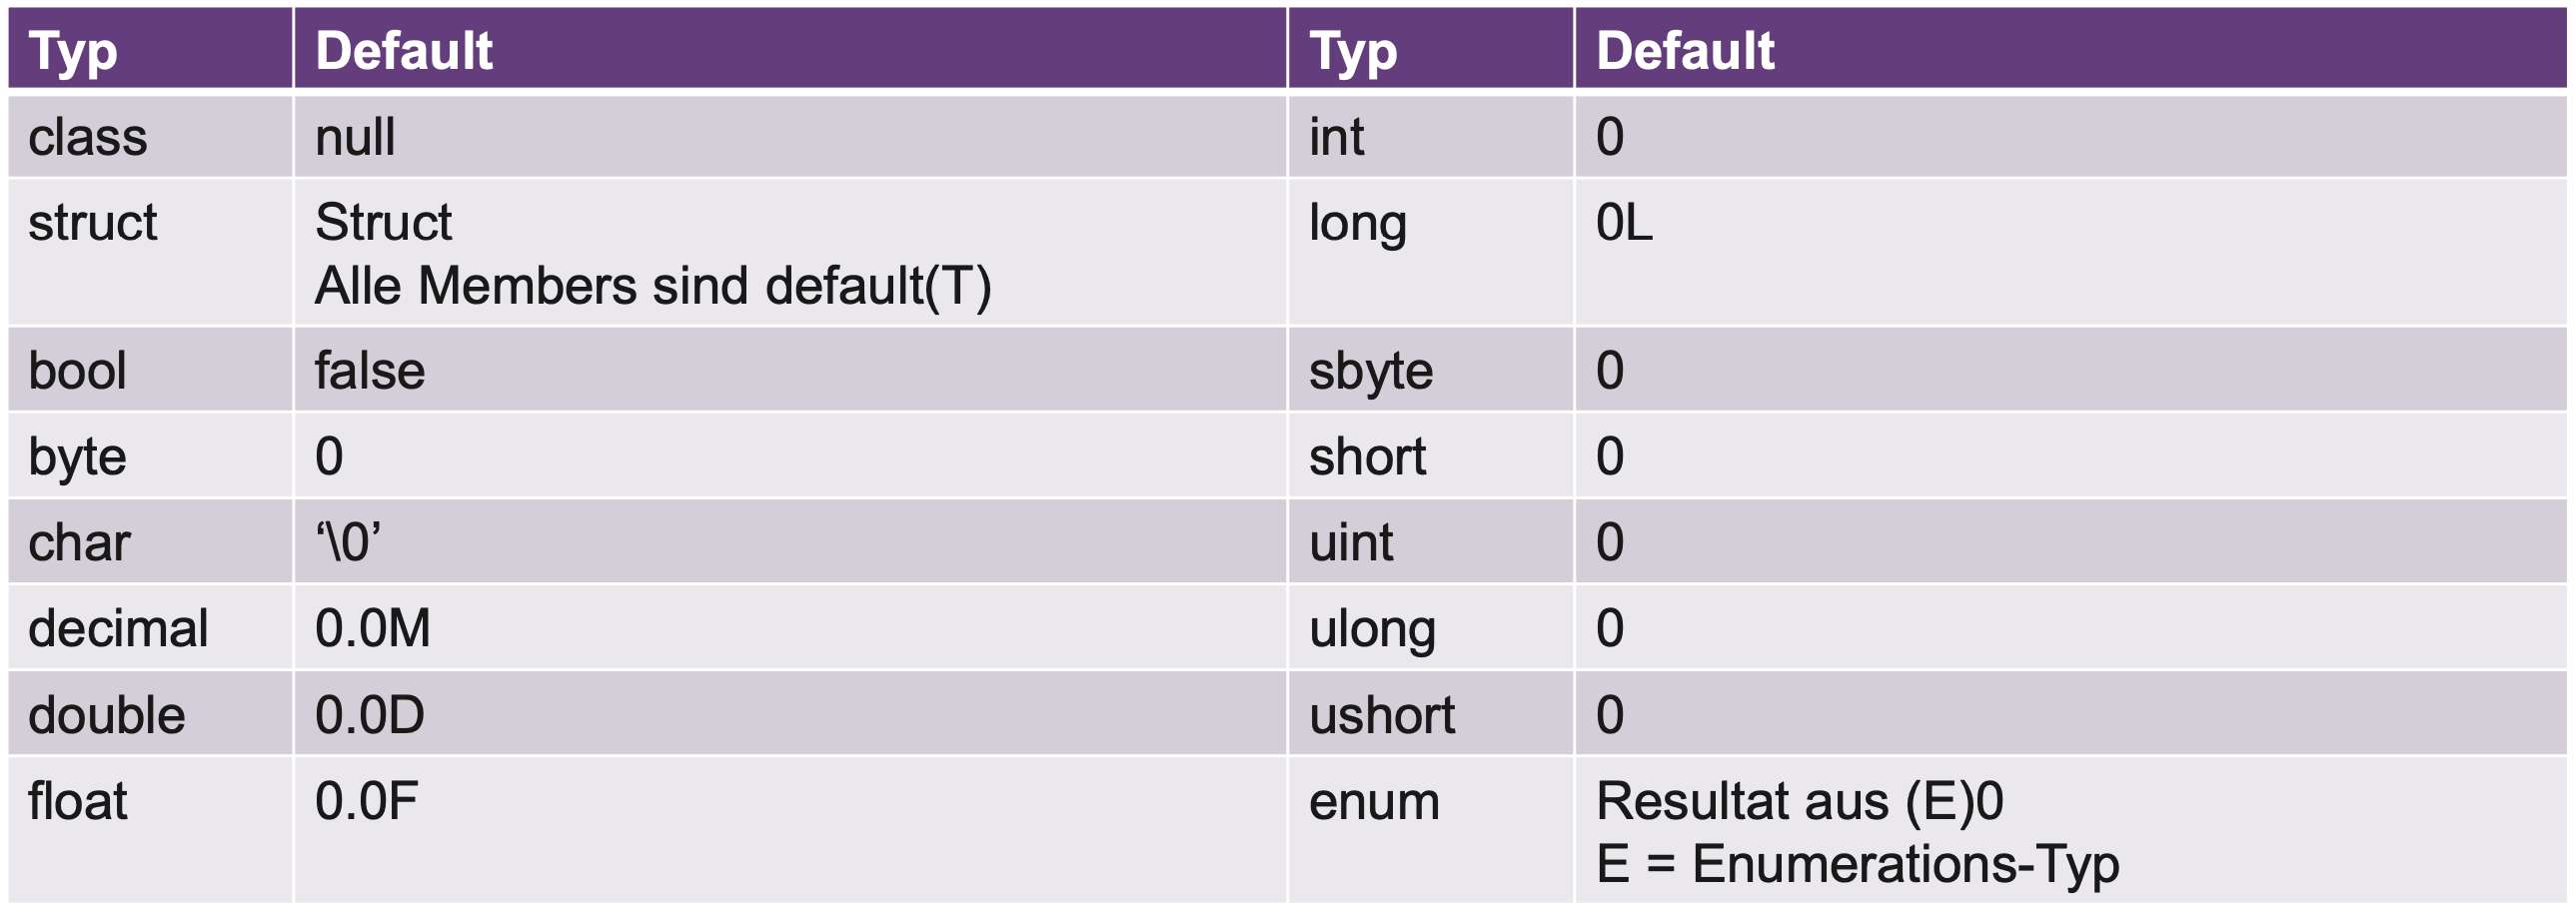
\includegraphics[scale=.18]{graphic/klassen/K&S_Standard-Werte.png}
\end{center}
\vspace{-8pt}

\subsubsection{Statische Konstruktoren}
\begin{itemize}
    \item Zwingend parameterlos
    \item Sichtbarkeit darf nicht angegeben werden
    \item Nur ein statischer Konstruktor erlaubt
    \item Wird genau einmal ausgeführt
    \item Kann nicht explizit aufgerufen werden
\end{itemize}

\subsubsection{Destruktoren}
\begin{itemize}
    \item Ermöglichen Abschlussarbeiten beim Abbau eines Objekts
    \item Nur bei Klassen erlaubt, bei Structs verboten
    \item Zwingend parameterlos / ohne Sichtbarkeit
    \item Nur ein Destruktor erlaubt
    \item Wird vom Garbage Collector aufgerufen
\end{itemize}

\begin{lstlisting}
class MyClass {
~MyClass() {
...
} }
\end{lstlisting}


\subsubsection{Initialisierungs Reihenfolge (ohne Vererbung)}
\begin{lstlisting}
class Base {
    private static int baseStaticValue = 0; private int baseValue = 0;
    static Base() { }
    public Base() { }
}

Base b1 = new Base();
// Base > baseStaticValue
// Base > Statischer Konstruktor
// Base > baseValue
// Base > Konstruktor

Base b2 = new Base();
// Base > baseValue
// Base > Konstruktor
\end{lstlisting}
\subsubsection{Initialisierungs Reihenfolge (mit Vererbung)}
\begin{lstlisting}
class Base {
    private static int baseStaticValue = 0; private int baseValue = 0;
    static Base() { }
    public Base() { }
}
class Sub : Base {
    private static int subStaticValue = 0; private int subValue = 0;
    static Sub() { }
    public Sub() { }
}

Sub s1 = new Sub();
// Sub > subStaticValue
// Sub > Statischer Konstruktor
// Sub > subValue
// Base > baseStaticValue
// Base > Statischer Konstruktor
// Base > baseValue
// Base > Konstruktor
// Sub > Konstruktor

Sub s2 = new Sub();
// Sub > subValue
// Base > baseValue
// Base > Konstruktor
// Sub > Konstruktor
\end{lstlisting}
\vspace{-8pt}
\begin{center}
    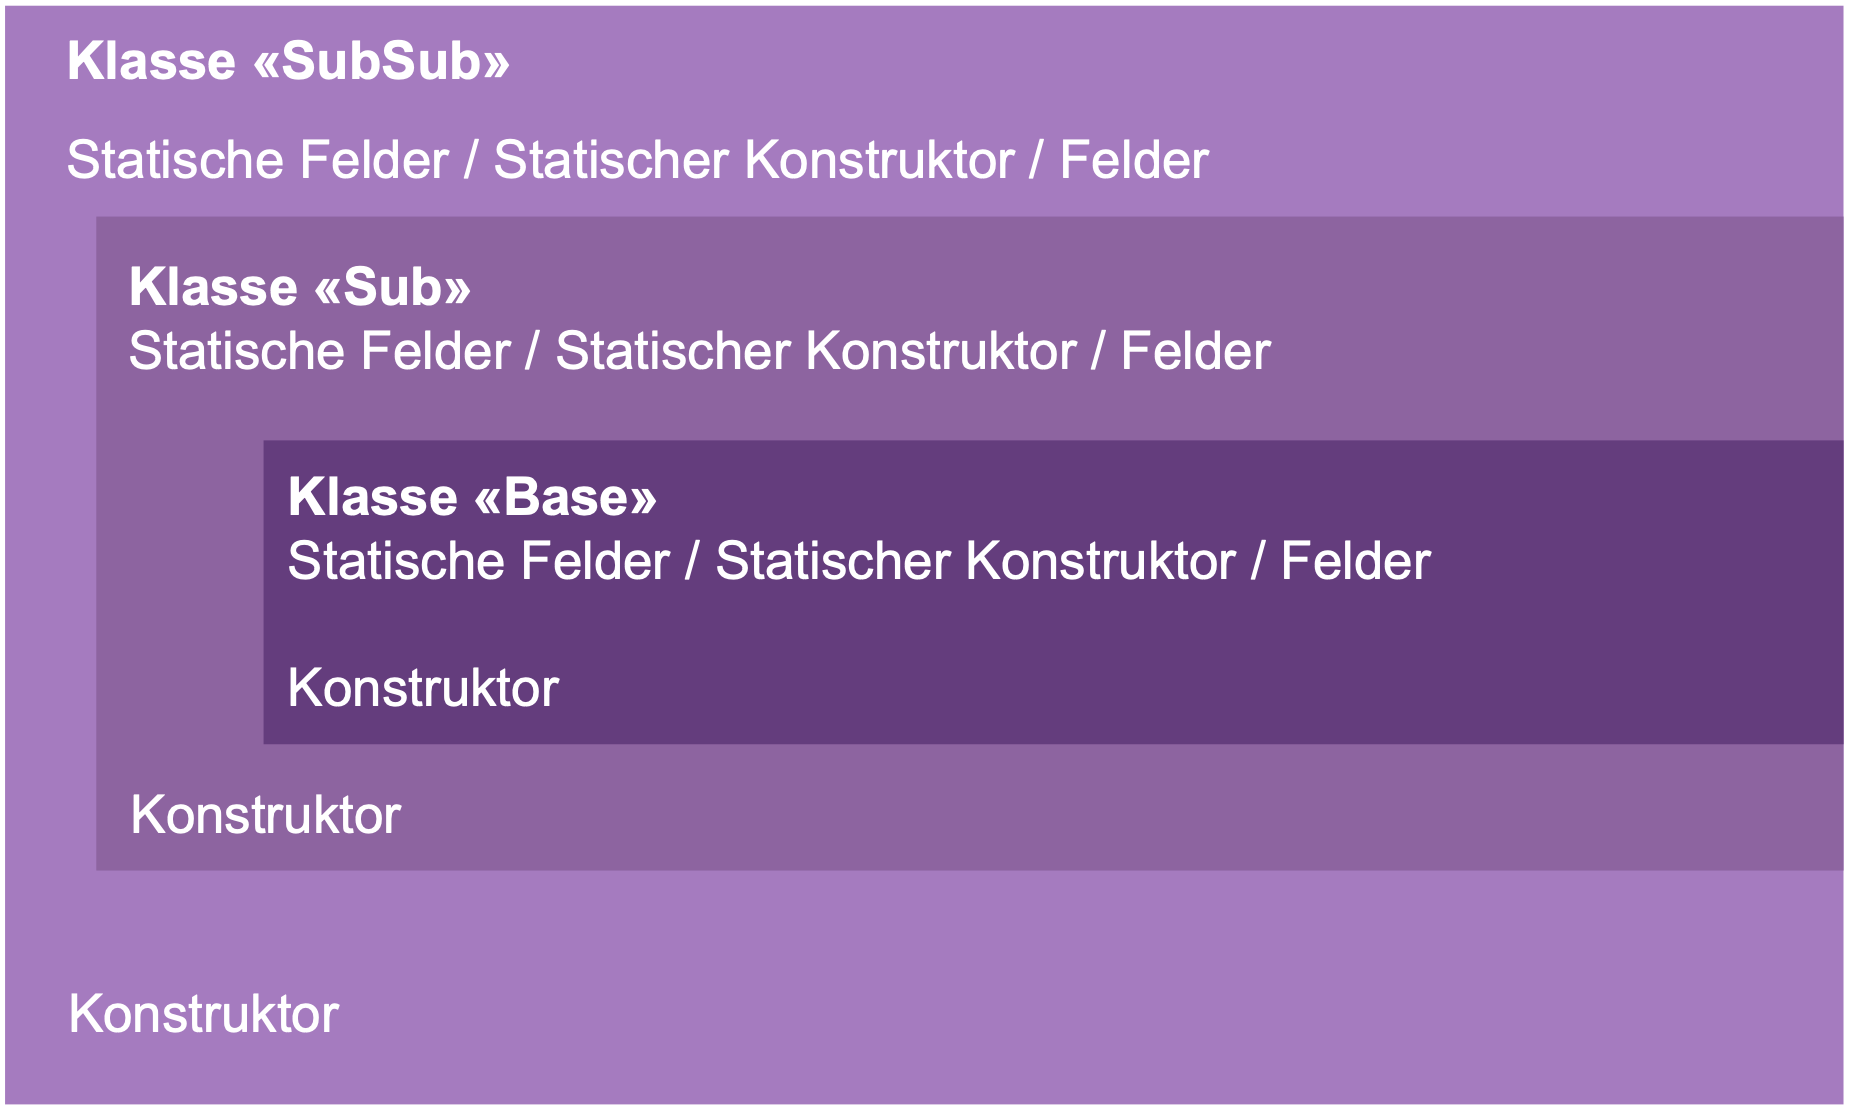
\includegraphics[scale=.2]{graphic/klassen/K&S_Init.png}
\end{center}
\vspace{-8pt}
\subsubsection{Konstruktoren in Ober- und Unterklasse}
\begin{center}
    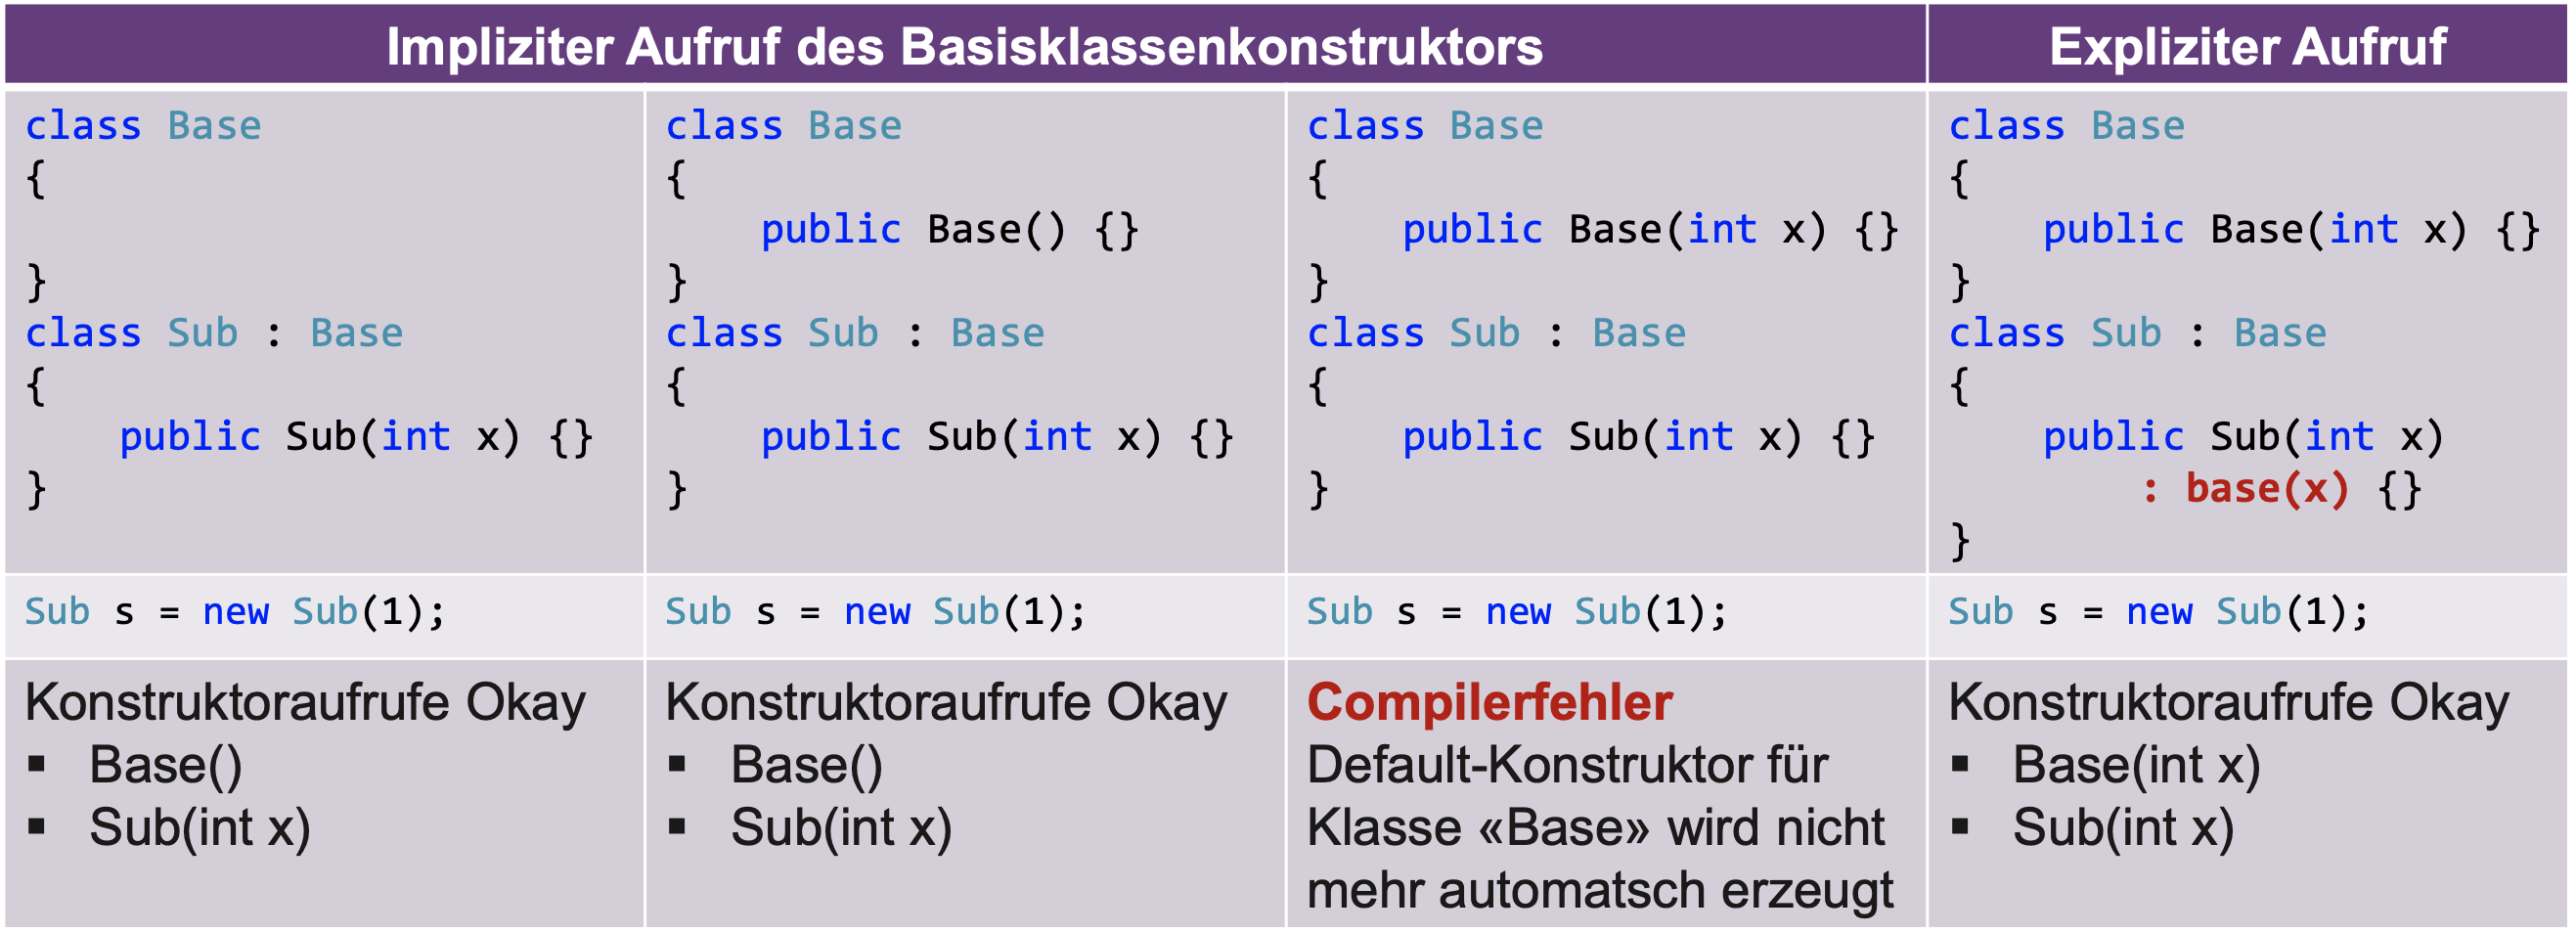
\includegraphics[scale=.19]{graphic/klassen/K&S_Konstruktoren in Ober- und Unterklasse.png}
\end{center}
\vspace{-8pt}


\subsection{Operator Overloading}
\begin{itemize}
    \item Methode muss «static» sein
    \item Schlüsselwort «operator» gefolgt von z.B. +
    \item Unäre Operatoren haben 1 Parameter
    \item Binäre Operatoren haben 2 Parameter
    \item Rückgabetyp ist frei wählbar
    \item Mindestens 1 Parameter muss vom Typ der enthaltenden Klasse sein
\end{itemize}

\begin{lstlisting}
class Point {
    private int x, y;
    public Point(int x, int y) { this.x = x; this.y = y; }

    public static Point operator ~(Point a) {
        return new Point(a.x * -1, a.y * -1); }

    public static Point operator +
        (Point a, Point b) {
        return new Point(a.x + b.x, a.y + b.y);
} }
\end{lstlisting}
\subsubsection{Unäre Operatoren}
\begin{lstlisting}
public static Point operator ~(Point a) {
    return new Point(a.x * -1, a.y * -1);
}

//Verwendung:
Point mcNeg = ~mc;
\end{lstlisting}
\subsubsection{Binäre Operatoren}
\begin{lstlisting}
public static Point operator +
        (Point a, Point b){
    return new Point(a.x + b.x, a.y + b.y);
}

//Verwendung:
Point mcSum = mc1 + mc2;
\end{lstlisting}

\subsection{Partielle Klassen}
\begin{itemize}
    \item Definition eines Typen in meheren Files
    \item Funktioniert mit: Klassen, Structs, Interfaces
    \item Alle Teile müssen die gleichen Sichtbarkeitsattribute haben (z.B. «public»)
    \item «partial» muss bei allen Teilen angemerkt sein
\end{itemize}

\begin{lstlisting}
// File1.cs
partial class MyClass {
    public void Test1() { }
}
// File2.cs
partial class MyClass {
    public void Test2() { }
}
\end{lstlisting}


\subsection{Partielle Methoden}

\begin{itemize}
    \item Trennung von Deklaration und Implementation einer Methode
    \item Ermöglicht Benutzer-definierte «Hooks» in generiertem Code
    \item Funktioniert in Klassen / Structs
    \item Rückgabewert muss «void» sein
    \item Implizit immer «private»
    \item Können «static» sein
\end{itemize}

\begin{lstlisting}
// File1.cs
partial class MyClass {
    public void Test1()
    {
        Test1Initialize();
/* ... */
Test1Cleanup(); }
    partial void Test1Initialize();
    partial void Test1Cleanup();
}
// File2.cs
partial class MyClass
{
    public void Test2() { }
    partial void Test1Initialize() { /* */ }
}
\end{lstlisting}

\newpage